\documentclass[a4paper,12pt,fleqn,oneside]{article} 
%\documentclass[a4paper,12pt,fleqn,oneside]{article} 	% Openright aabner kapitler paa hoejresider (openany begge)

%===== Projekt konstanter =====
\newcommand{\kursusTitel}{Semesterprojekt 3}
\newcommand{\linje}{E/IKT}
\newcommand{\semester}{3}
\newcommand{\system}{Beer Pong Table}
\newcommand{\rapportType}{Proces}
\newcommand{\gruppeNr}{7}
\newcommand{\vejleder}{Martin Ansbjerg Kjaer}
\newcommand{\afleveringsdato}{19. december 2018}

%%%% PAKKER %%%%
% ¤¤ Oversaettelse og tegnsaetning ¤¤ %
\usepackage[utf8]{inputenc}					% Input-indkodning af tegnsaet (UTF8)
\usepackage[english, danish]{babel}			% Dokumentets sprog
\usepackage[T1]{fontenc}					% Output-indkodning af tegnsaet (T1)
\usepackage{ragged2e,anyfontsize}			% Justering af elementer

% ¤¤ Figurer og tabeller (floats) ¤¤ %
\usepackage{wrapfig}                        % text wrapping
\usepackage{graphicx} 						% Haandtering af eksterne billeder (JPG, PNG, PDF)
\usepackage{caption}
\usepackage{subcaption}
\usepackage{multirow}
% Fletning af raekker og kolonner (\multicolumn og \multirow)
\usepackage{makecell}                       % Line breaks i tabelceller med \makecell{bla bla \\ bla bla}
\usepackage{colortbl} 						% Farver i tabeller (fx \columncolor, \rowcolor og \cellcolor)
\usepackage[dvipsnames,table,longtable,x11names]{xcolor}

%Tabel automatisk ny linje
\usepackage{array}
\newcolumntype{L}[1]{>{\raggedright\let\newline\\\arraybackslash\hspace{0pt}}m{#1}}
\newcolumntype{C}[1]{>{\centering\let\newline\\\arraybackslash\hspace{0pt}}m{#1}}
\newcolumntype{R}[1]{>{\raggedleft\let\newline\\\arraybackslash\hspace{0pt}}m{#1}}

% Definer farver med \definecolor. Se mere: http://en.wikibooks.org/wiki/LaTeX/Colors
\usepackage{flafter}						% Soerger for at floats ikke optraeder i teksten foer deres reference
\let\newfloat\relax 						% Justering mellem float-pakken og memoir
\usepackage{float}							% Muliggoer eksakt placering af floats, f.eks.
\usepackage{afterpage}
%\usepackage{scrextend}                      % labeling lister
\usepackage{chngcntr} % kontroller nummerering af floats
\counterwithin{figure}{section} % sæt nummerering efter sektion
\counterwithin{table}{section} % sæt nummerering efter sektion

% ¤¤ Matematik mm. ¤¤
\usepackage{amsmath,amssymb,stmaryrd} 		% Avancerede matematik-udvidelser
\usepackage{mathtools}						% Andre matematik- og tegnudvidelser
\usepackage{textcomp}                 		% Symbol-udvidelser (f.eks. promille-tegn med \textperthousand )
\usepackage{siunitx}						% Flot og konsistent praesentation af tal og enheder med \si{enhed} og \SI{tal}{enhed}
\sisetup{output-decimal-marker = {,}}		% Opsaetning af \SI (DE for komma som decimalseparator)

% ¤¤ Misc. ¤¤ %
\usepackage{listings}						% Placer kildekode i dokumentet med \begin{lstlisting}...\end{lstlisting}

%Custom C Code Style
\lstdefinestyle{customc}{
    breaklines=true,
    language=C,
    basicstyle=\small\sffamily,
    numbers=left,
    numberstyle=\tiny\color{gray},
    frame=tb,
    columns=fullflexible,
    showstringspaces=false,
    keywordstyle=\bfseries\color{green!40!black},
    commentstyle=\itshape\color{purple!40!black},
    identifierstyle=\color{blue},
    stringstyle=\color{orange},
}


\usepackage{blindtext}
\usepackage{lipsum}							% Dummy text \lipsum[..]
\usepackage[shortlabels]{enumitem}			% Muliggoer enkelt konfiguration af lister
\usepackage{pdfpages}						% Goer det muligt at inkludere pdf-dokumenter med kommandoen \includepdf[pages={x-y}]{fil.pdf}
\usepackage[bottom]{footmisc}               % Saetter footnotes i bunden af siden
\pdfoptionpdfminorversion=6					% Muliggoer inkludering af pdf dokumenter, af version 1.6 og hoejere
\pretolerance=2500 							% Justering af afstand mellem ord (hoejt tal, mindre orddeling og mere luft mellem ord)


%%%% BRUGERDEFINEREDE INDSTILLINGER %%%%

\linespread{1,1}							% Linie afstand

% ¤¤ Visuelle referencer ¤¤ %
\usepackage[colorlinks,pdfencoding=auto]{hyperref}			% Danner klikbare referencer (hyperlinks) i dokumentet.
\hypersetup{colorlinks = true,				% Opsaetning af farvede hyperlinks (interne links, citeringer og URL)
    linkcolor = black,
    citecolor = black,
    urlcolor = black
}

%%%% TODO-NOTER %%%%
\usepackage[danish, colorinlistoftodos]{todonotes}
%\usepackage[colorinlistoftodos]{todonotes}

%%%% TABEL BAGGRUNDSFARVER %%%%
\definecolor{aublueclassic}{RGB}{0,61,115}
\definecolor{aubluedark}{RGB}{0,37,70}
\definecolor{aucyan}{RGB}{225,248,253}
%\definecolor{aucyan}{RGB}{55,160,203}
\definecolor{aucyandark}{RGB}{0,62,92}
\definecolor{lightGray}{RGB}{153,153,153}
\definecolor{darkGray}{RGB}{119,119,119}
\definecolor{khaki}{RGB}{240,230,140}
\definecolor{lavender}{RGB}{230,230,250}

%indentering af section
\usepackage{changepage}

%Code highlighting
\usepackage{minted}

%%%% Tabs %%%%
\usepackage{tabto}
\NumTabs{10}

%%%% REFERENCE TIL SECTION-NAME %%%%
\usepackage{nameref}
\newcommand*{\fullref}[1]{\textbf{\ref{#1} \nameref{#1}}} % One single link

%sidehoved
\usepackage{fancyhdr}
\usepackage{lastpage}

%referer til afsnit i andre dokumenter
\usepackage{xr}

\externaldocument[arch:]{aux_files/Arkitektur}
\externaldocument[accepttestspec:]{aux_files/Accepttestspecifikation}
\externaldocument[hwdesign:]{aux_files/HardwareDesign}
\externaldocument[analyse:]{aux_files/Analyse}
\externaldocument[integration:]{aux_files/Integrationstest}
\externaldocument[kravspec:]{aux_files/Kravspecifikation}
\externaldocument[modultest:]{aux_files/Modultest}
\externaldocument[proces:]{aux_files/Procesdokument}
\externaldocument[swdesign:]{aux_files/Softwaredesign}

%%%% biblatex %%%%
\usepackage[backend=bibtex,style=ieee]{biblatex}
\bibliography{Litteratur} 

%%%% KRAV numerering %%%%

\newcounter{req} \setcounter{req}{0}
\newcounter{subreq}[req] \setcounter{subreq}{0}
 
\renewcommand{\thereq}{\arabic{req}}
\renewcommand{\thesubreq}{\arabic{req}.\arabic{subreq}}
 
\newenvironment{req}[1]%
{
\refstepcounter{req}{K\thereq}}{}
\newenvironment{subreq}[1]%
{
\refstepcounter{subreq}{\noindent K\thesubreq}}{}


%%%% paragraph %%%%
%\usepackage{titlesec}
%\setcounter{secnumdepth}{4}

%\titleformat{\paragraph}
%{\normalfont\normalsize\bfseries}{\theparagraph}{1em}{}
%\titlespacing*{\paragraph}
%{0pt}{3.25ex plus 1ex minus .2ex}{1.5ex plus .2ex}

% ========== PAKKER DER SKAL LOADES TIL SIDST ==================
%\usepackage{xcolor}
%\usepackage{listings}
\usepackage{csquotes}           %så holder bilatex kæft
\usepackage{subfiles}


%%EDS SHIT
\PassOptionsToPackage{unicode=true}{hyperref} % options for packages loaded elsewhere
\PassOptionsToPackage{hyphens}{url}
%
\usepackage{lmodern}
\usepackage{amssymb,amsmath}
\usepackage{ifxetex,ifluatex}
\ifnum 0\ifxetex 1\fi\ifluatex 1\fi=0 % if pdftex
  \usepackage[T1]{fontenc}
  \usepackage[utf8]{inputenc}
  \usepackage{textcomp} % provides euro and other symbols
\else % if luatex or xelatex
  \usepackage{unicode-math}
  \defaultfontfeatures{Ligatures=TeX,Scale=MatchLowercase}
\fi
% use upquote if available, for straight quotes in verbatim environments
\IfFileExists{upquote.sty}{\usepackage{upquote}}{}
% use microtype if available
\IfFileExists{microtype.sty}{%
\usepackage[]{microtype}
\UseMicrotypeSet[protrusion]{basicmath} % disable protrusion for tt fonts
}{}
\IfFileExists{parskip.sty}{%
\usepackage{parskip}
}{% else
\setlength{\parindent}{0pt}
\setlength{\parskip}{6pt plus 2pt minus 1pt}
}
\usepackage{hyperref}
\hypersetup{
            pdfborder={0 0 0},
            breaklinks=true}
\urlstyle{same}  % don't use monospace font for urls
\usepackage{longtable,booktabs}
% Fix footnotes in tables (requires footnote package)
\IfFileExists{footnote.sty}{\usepackage{footnote}\makesavenoteenv{longtable}}{}
\setlength{\emergencystretch}{3em}  % prevent overfull lines
\providecommand{\tightlist}{%
  \setlength{\itemsep}{0pt}\setlength{\parskip}{0pt}}
% Redefines (sub)paragraphs to behave more like sections
\ifx\paragraph\undefined\else
\let\oldparagraph\paragraph
\renewcommand{\paragraph}[1]{\oldparagraph{#1}\mbox{}}
\fi
\ifx\subparagraph\undefined\else
\let\oldsubparagraph\subparagraph
\renewcommand{\subparagraph}[1]{\oldsubparagraph{#1}\mbox{}}
\fi

% set default figure placement to htbp
\makeatletter
\def\fps@figure{htbp}
\makeatother

\def\titlename{Proces}

\begin{document}

%===============FORSIDE======================
\begin{titlepage}

\newcommand{\HRule}{\rule{\linewidth}{0.5mm}} % Defines a new command for the horizontal lines, change thickness here

\center % Center everything on the page
 
%----------------------------------------------------------------------------------------
%	HEADING SECTIONS
%----------------------------------------------------------------------------------------

\textsc{\LARGE Aarhus Universitet }\\[0.3cm] % Name of your university/college
\textsc{\Large 3. Semesterprojekt }\\[0.3cm]
\textsc{\Large Gruppe 7 }\\[0.5cm] % Major heading such as course name
 % Minor heading such as course title

%----------------------------------------------------------------------------------------
%	TITLE SECTION
%----------------------------------------------------------------------------------------

\HRule \\[0.4cm]
{ \huge \bfseries \titlename}\\[0.03cm]{Beerpong Table} % Title of your document
\HRule \\[1.5cm]

 
%----------------------------------------------------------------------------------------
%	AUTHOR SECTION
%----------------------------------------------------------------------------------------

\begin{minipage}{0.4\textwidth}
\begin{flushleft} \small
\emph{Gruppemedlemmer:}
\\Aaron Becerril Sanchez\\ (AU592162)
\\Edward Hestnes Brunton\\ (AU576633)
\\Marcus Gasberg\\ (AU587414) 
\\Martin Gildberg Jespersen\\ (AU593618) 
\\Martin Lundberg\\ () 
\\Mathias Magnild Hansen\\ (AU520773)
\\Nikolaj Holm Gylling\\ (AU592243)
\\Tristan Moeller\\ (AU569046)
\end{flushleft}
\end{minipage}
~
\begin{minipage}{0.4\textwidth}
\begin{flushright} \small
\emph{Vejleder:} \\
Martin Ansbjerg Kjær \\ Civ. Ing., Ph.D., Adjunkt % Supervisor's Name
\end{flushright}
\end{minipage}\\[1cm]

% If you don't want a supervisor, uncomment the two lines below and remove the section above
%\Large \emph{Author:}\\
%John \textsc{Smith}\\[3cm] % Your name

%----------------------------------------------------------------------------------------
%	DATE SECTION
%----------------------------------------------------------------------------------------

{\large December 2018}\\[1cm] % Date, change the \today to a set date if you want to be precise

%----------------------------------------------------------------------------------------
%	LOGO SECTION
%----------------------------------------------------------------------------------------


\includegraphics{Setup/graphics/AU.png}\\[1cm] %Logo

\vfill
\end{titlepage}
\subfile{Processdokument/Versionshistorik/Versionshistorik.tex}\newpage
\tableofcontents
\newpage

\section{Forord}
Dette dokument er skrevet af PRJ3 gruppe 7, der en projektgruppe bestående af 3. semesters E- og IKT-studerende fra Aarhus Universitets. Dette dokument er udarbejdet som en beskrivelse af den proces, gruppen har været igennem under hele semesteret og har til formål, at være en opsummering og sammenbringelse af procesrelateret information for, hvem end det må interessere. Det forudsætter for at forstå dette dokument, at i hvert fald Projekt Introduktionen og noget af Kravspecifikationen er læst forud for dette. Derudover fungere dette dokument som en uddybning af Proces afsnittet i rapporten.

\section{Indledning}
I dokumentet vil der være en beskrivelse af alt det arbejde, der er lavet i forbindelse med processen til udvikling af projektet. Der vil være en beskrivelse af, hvordan gruppen blev dannet, og den samarbejdsaftale, der blev lavet, som kontrakt for gruppen. Det beskrives også hvilket udviklingsredskab eller udviklingmetode, der blev valgt, hvordan projektet blev ledet og den arbejdsfordeling, der har været mellem medlemmerne af gruppen. Der vil også blive beskrevet, hvordan forskellig planlægning blev lavet i gruppen, hvordan møderne blev afholdt, og hvordan eventuelle konflikter er håndteret.

\section{Gruppedannelse}
På 3. semester projektet var det muligt at ønske, et givent antal personer, man ønskede at danne gruppe med. I gruppen havde 5 af de IKT-studerende ønsket at være på hold sammen, hvilket de kom. De blev så sat sammen med 2 E-studerende, hvilket gav en stærk overvægt af interesse for software i gruppen. Da der i hver gruppe må være max 8 studerende, så blev gruppen kort tid efterspurgt om de havde plads til en IKT-studerende mere. Dette takkedes selvfølgelig ja til. Nu var der altså en overvægt på 6 IKT-studerende til 2 E-studerende, men da meget af den elektroniske baggrund var  den samme for begge parter, blev der lavet en aftale om at studieretning ikke havde fast betydning for, hvad man kom til at arbejde med. Et værktøj der blev anvendt på første og andet semester, kaldet \textit{Insights Profiler}, blev efter gruppedannelse kort brugt til at give et overblik over, hvilke personligheder, gruppen bestod af. Den blev ikke brugt til at danne grupperne ud fra, men den gav ligesom et overblik over sammensætningen af gruppen og kompetencer og svagheder. I
følgende tabel ses \textit{Insights} sammensætningen af gruppen, der kan sammenlignes med figur\footnote{https://www.insights.com/dk/produkter/insights-discovery/} \ref{fig:group_types}.
\begin{table}[H]
\centering
\begin{tabular}{|L{0.2\textwidth}|L{0.2\textwidth}|L{0.4\textwidth}|}
\hline
\textbf{Navn} & \textbf{Farve} & \textbf{Type} \\ \hline
Nikolaj & Blå & Reformerende Observatør  \\ \hline
Tristan & Gul & Inspirerende Motivator\\ \hline
Mathias & Grøn & Supporter \\ \hline
Edward & Blå & Reformerende Observator \\ \hline
Martin G.J. & Blå  & Observatør \\ \hline
Martin F. & Lilla & Reformator  \\ \hline
Aaron & Orange & Motivator \\ \hline
Marcus & Gul & Inspirator \\ \hline
\end{tabular}
\caption{Sammensætning af Insights typer i gruppen}
\label{table_group_types}
\end{table}

\begin{figure}[H]
    \centering
    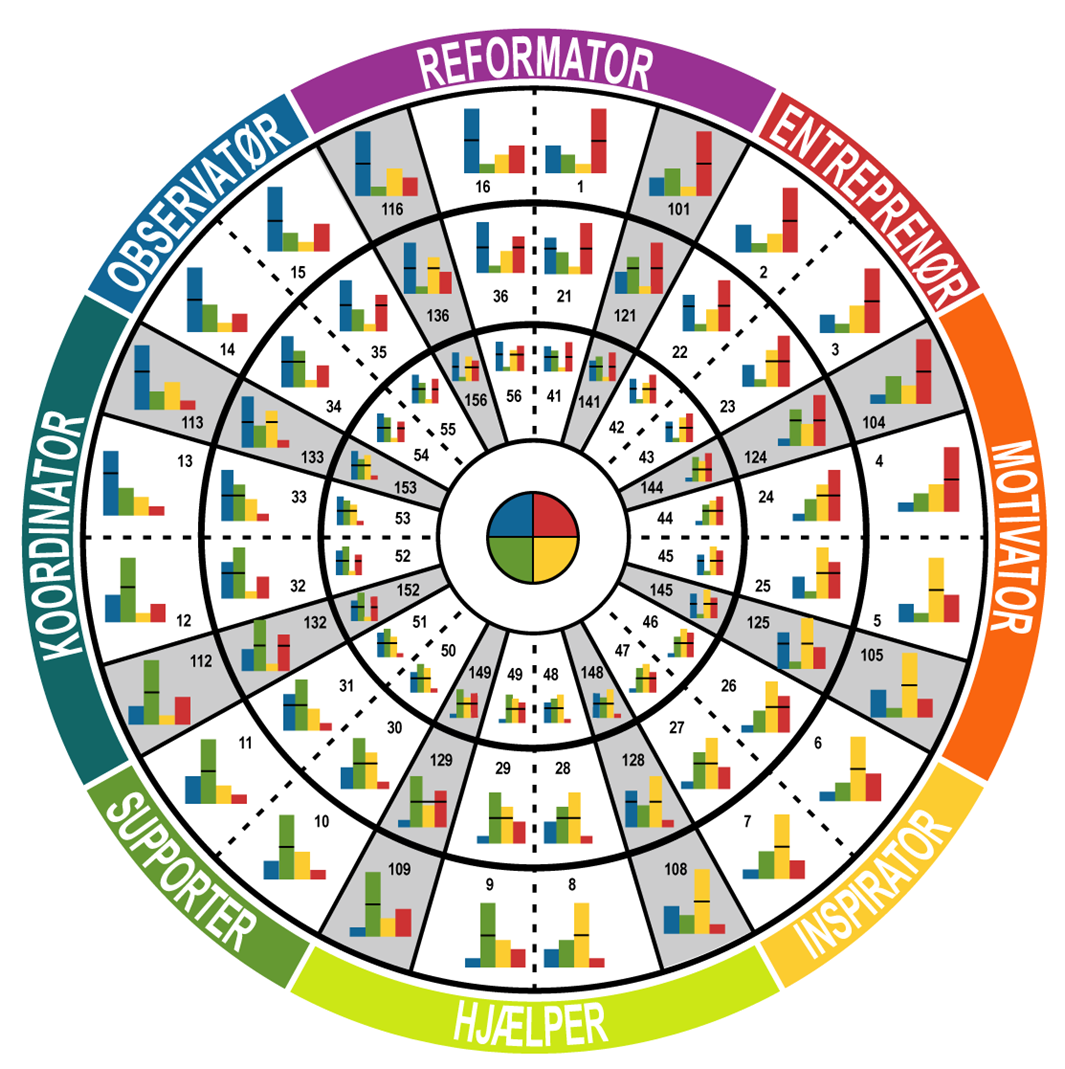
\includegraphics[width=0.5\textwidth]{Processdokument/graphics/type_cirkel.png}
    \caption{De forskellige Insights typer i gruppen}
    \label{fig:group_types}
\end{figure}

\section{Udviklingsforløb}
\subsection{Introduktion}
Dette afsnit omhandler den generelle beskrivelse af udviklingforløbet på PRJ3. Før der laves en beskrivelse af, hvordan forløbet har været i gruppen, er det relevant at se på, hvad projekt oplægget siger om det\footnote{PRJ3 - Semesterprojekt 3
Beskrivelse af indhold og standardprojekt}. I indledning af projekt oplægs dokumentet er der blandt andet opstillet følgende fire punkter.
\begin{enumerate}
    \item Implementering og test af et udviklingsprojekt med både HW og SW, der integrerer semesterets kurser.
    \item Anvendelsen af processer og metoder kendt fra projektet på 2. semester, men anvendt iterativt over alle faser.
    \item Samarbejde i grupper med både HW og SW udviklerroller
    \item Iterativ arbejdsmetode, SCRUM, orienteret mod at udvikle nye produkter baseret på HW og SW.
\end{enumerate}
Af denne liste ses det, at i relation til udviklingsforløbet skal beskrives, hvordan der er blevet anvendt processer og metoder fra projektet på 2. semester, men i endnu højere grad, hvordan der er blevet arbejdet iterativt i forbindelse med Scrum.

\subsection{Scrum}
Det første arbejde, der blev lavet, der har med Scrum at gøre, var at lave en definition af, hvordan Scrum skulle anvendes i gruppen. Der blev her udarbejdet et dokument som forslag til, hvordan Scrum kunne anvendes i gruppen. Forslaget blev gennemgået fælles i gruppen, hvor der blev lavet rettelser, tilføjelser og fjernelser. Der var nu et udkast til, hvilke Scrum relaterede opgaver, der var i gruppen, hvordan møderne skulle afholdes og hvilke redskaber, der skulle bruges til at Scrum kunne faciliteres. Som overblik for den tiltænkte anvendelse af Scrum, henvises der til figur\footnote{https://www.testingexcellence.com/overview-of-scrum-agile-development-methodology/} \ref{fig:scrum_process}. Det er dog vigtigt, at være opmærksom på, at det ikke er præcist denne måde, Scrum blev anvendt på, da forskellige faktorer gjorde dette umuligt. 
\begin{figure}[H]
    \centering
    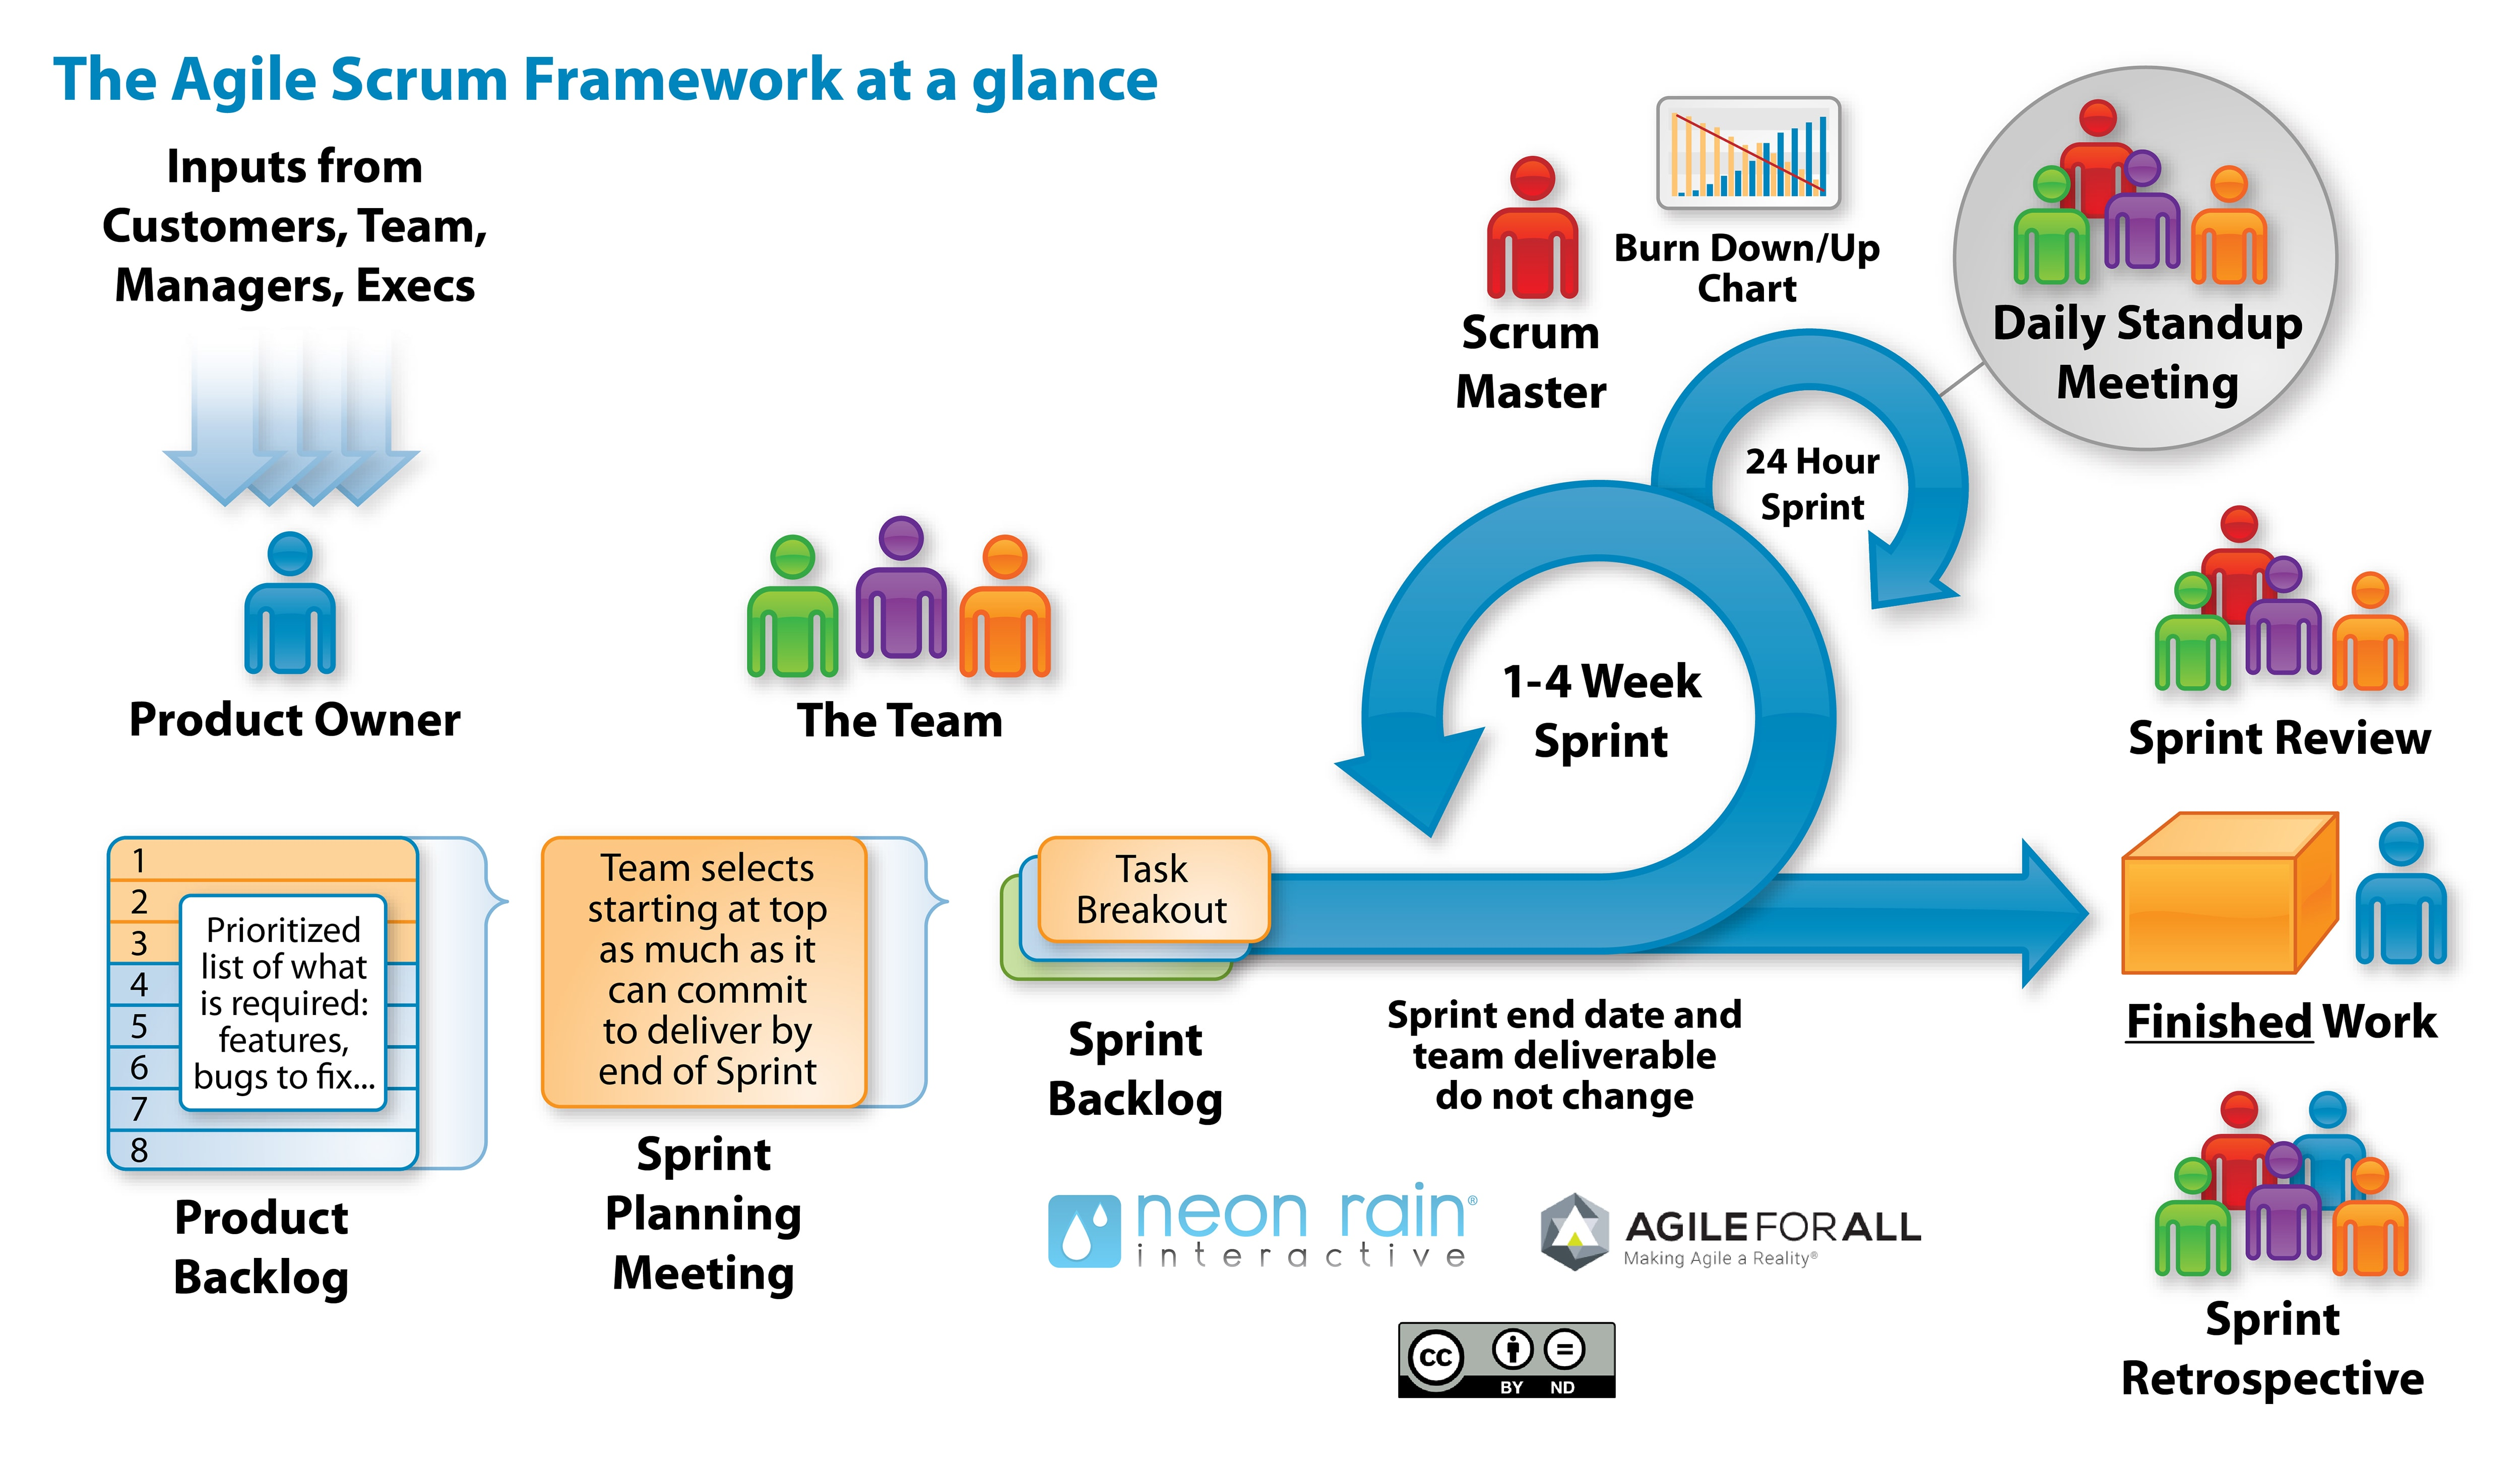
\includegraphics[width=\textwidth]{Processdokument/graphics/scrum_process_afa_5000.jpg}
    \caption{Procesbeskrivelse for Scrum}
    \label{fig:scrum_process}
\end{figure}
De følgende underafsnit fungere, som gennemgang af det dokument, der blev udarbejdet i starten, men også som beskrivelse for, hvordan Scrum blev anvendt anderledes end det ses af figur \ref{fig:scrum_process}.
\subsubsection{Sprints}
Det blev besluttet at hvert Sprint skulle have en varighed af 2 uger. Grunden til at lige netop denne varighed blev besluttet, var at, hvis det blev kortere, ville der blive brugt for lang tid på Sprintplanlægning og Sprintreview. Varede Sprintet derimod længere, ville det også blive et problem, da det ville kræve, at langt flere tasks skulle planlægges,  end vi troede vi var i stand til, og det ville også stille højere krav til evnen til at estimere, hvor lang tid hver task tager.  

\subsubsection{Rollerne i Scrum}
Her laves en gennemgang af de klassiske roller, der er i Scrum og hvordan de blev realiseret i projektgruppen. 
\\\\\textbf{Scrum Master}
\\Rollen som Scrum Master er en vigtig rolle, da han faciliterer Scrum i projektgruppen. Det er samtidig også den sværeste rolle, da ingen i gruppen havde erfaring med at være Scrum Master eller Scrum i det hele taget på forhånd. Det blev derfor også hurtigt besluttet, at man i gruppen bestræbede sig i så høj grad som muligt for, at denne rolle gik på tur efter hvert sprint, så alle fik den erfaring. For selve rollen blev det besluttet, at han skulle stå for at fjerne interne eller eksterne forhindring for gruppen, så gruppen fungere produktivt og funktionelt. Det er også ham, der står for varetagelse af Scrum-boardet, der beskrives i afsnit \ref{scrum_tools} om Redskaber.
\\\\\textbf{Product Owner}
\\Som Product Owner har man ansvaret for, at bestemme, hvad der skal laves på produktet, samt hvad prioritet de forskellige arbejdsopgaver har. Dette beslutter han ud fra kommunikation med forskellige eksterne parter. Denne rolle er modificeret til at passe til et semesterprojekt, da gruppen i princippet er deres egen Product Owner, og hvor den mest eksterne indflydelse er fra projektvejlederen. Denne rolle varetages derfor af hele gruppen og tildels projektvejlederen. Det er også værd at nævne at prioritering af arbejdsopgaver laves ud fra en fælles risikoanalyse.
\\\\\textbf{Team Member}
\\Alle i gruppen fungere som Team Member, da alle er en del af Teamet og bliver nødt til at have arbejdsopgaver, der arbejder frem mod færdiggørelsen af projektet. Det vil altså også sige, at bare fordi man er Scrum Master, så er man ikke frasagt arbejdsopgaver, der ligger udenfor scrum masterens rolle. Det er derudover også vigtigt for gruppen, at grundet den fordeling af studieretninger  (6 IKT- og 2 E-studerende), der er i gruppen, ikke bliver givet arbejdsopgaver ud fra kompetencer. Dette virker måske selvmodsigende af Scrum, men det er et nødvendigt onde, da de få E-studerende ellers ville stå med rigtig mange opgaver.
\subsubsection{Scrum relaterede møder}
Henvises der til figur \ref{fig:scrum_process}, så kan der hives 4 møder ud: Daily Standup Meeting, Sprintplanlægning, Sprint Retrospective og Sprint Review. Da alle gruppens medlemmer samtidigt fungere som studerende på Aarhus Universitet, var det allerede fra en start tydeligt, at det ville være urealistisk at holde et møde om dagen. Efter lidt gennemgang af kalenderen, blev det fundet, at de eneste tidspunkter, det var muligt for begge studieretninger at mødes, var mandag eftermiddag og torsdag morgen. Det blev derfor besluttet, at der inden hvert møde var et kort Standup Meeting, der havde til formål at opdatere alle parter om, hvad de andre lavede og hvor langt de var. Med to dage at vælge ud fra, blev det også tydeligt, at der hver anden uge, efter hvert sprint, måtte laves et samlet møde for Sprint-Retrospektiv,-Review og Planlægning. 

\subsubsection{Redskaber} \label{scrum_tools}
Det vigtigste redskab i anvendelsen af Scrum i gruppen var det såkaldte Scrum-board. Det var denne, der skulle fungere som Product Backlog, Sprint Backlog og som oversigt over alle tasks. Hvad de indeholdte, hvem der var tildelt tasken, deres estimerede varighed, samt tiden der var brugt på den. Det første valg i forhold til Scrumboard var hjemmesiden Trello, men det blev dog hurtigt tydeligt, at den ikke tilbød alle de ønskede funktioner (Uden betaling i hvert fald). Kort tid efter var der dog en introduktion til Redmine, til facilitering af Scrum, og der blev hurtigt lavet en transition over til denne. Transitionen til Redmine fandt sted i 2. sprint. 
\\Noget andet godt ved Redmine er også, at det har en integreret Wiki, som kan anvendes til at nedskrive information omkring sprintene, og deres planlægning, mål og retrospektiv. Det er denne wiki, de følgende sektioner tager udgangspunkt i. I Redmine er der også mulighed for at oprette repositories til de forskellige delprojekter af projektet.

\subsection{Erfaringer med Scrum}\label{sec:experiences_w_scrum}
\subsubsection{Introduktion}
Som sagt er Scrum en ny arbejdsmetode for alle i gruppen, men ikke blot det, der er også en masse nye teknologier, der skulle afprøves og stiftes erfaring med. Samtidig med at man lærer disse teknologier at kende, skal man også lærer at arbejde iterativt og effektivt med Scrum. Heldigvis er retrospektiver et rigtig godt redskab til at lære fra de Sprints man netop har gennemført. Dette afsnit gennemgår nogle af de erfaringer, der er blevet gjort i løbet af processen omkring Scrum. Både hvad der har fungeret, men også hvad der ikke har fungeret.

\subsubsection{Sprint 1}
Det indledende sprint i projektet. Dette sprint kan mest af alt beskrives, som værende meget kaotisk, da man prøver at tage beslutninger uden egentlig at have erfaringer omkring Scrum. Samtidig har man ikke et egentlig projekt at arbejde på, og man skal indbyrdes lære hinanden at kende. Der er mange beslutninger at tage i sprintet, og samtidig skal der skabes en rytme for, hvordan man gør tingene i gruppen. 
\\Dette afspejles også i retrospektivet, hvor der blandt andet nævnes bedre kommunikation og planlægning i gruppen, samtidig med at Scrum Master rollen skulle træde mere i fokus. 

\subsubsection{Sprint 2}
Dette sprint var, hvor Scrum for alvor begyndte at træde i kraft, da der begyndtes på første iteration af det første store dokument, Kravspecifikationen. Kravsspecifikationen indeholder mange underopgaver, som f.eks. use cases, aktør-kontekst diagram og forskellige ikke funktionelle krav. Derudover blev der også begyndt på tidsplan, risikoanalyse og Accept testspecifikation, samtidig med at der skulle laves en opsætning af både Redmine og Overleaf. I bedste scrum stil bestræbedes der efter at have så mange små opgaver som muligt, men der var dog enighed om, at denne opgave ikke lykkedes særligt godt og der manglede flere tasks. Det hang uløseligt også sammen med at sprintet ikke var planlagt godt nok, og der ikke var sat et specifikt mål for hvad der skulle nås. En anden ting der bidragede til dette, var at der ikke var lavet tidsestimering på opgaverne, så der var intet overblik over, hvor lang tid opgaverne ville tage. Noget der dog lykkedes meget godt var, hvordan der holdtes stand-up meeting, og hvordan der kommunikeredes. Bagefter blev der også gennemgået de vigtigste ting de enkelte i teamet havde arbejdet på, så alle havde en klar forståelse af, hvordan projektet fungerede. 

\subsubsection{Sprint 3}
Når nu man planlægger et sprint, så er det vigtigt, at der tages hensyn til om, der er vigtige deadlines, som der tages hånd om i planlægningen. I det her sprint fejlede gruppens overblik over, hvad der skulle være færdigt til første review . F.eks. blev der ret sent fundet ud af, at den første version af Systemarkitekturen skulle med til review, og derfor fik få i teamet relativt tunge opgaver oveni i de eksisterende. I gruppen var man dog god til at reviewe de arbejdsopgaver, der var lavet til møderne, så kvaliteten ikke haltede påtrods af presset. I retrospektivet for dette sprint var det tydeligt, at dette også var problematisk i sprintet. Derudover var der også enighed om at de store tasks skulle være opdelt i mindre tasks, da andre færdiggjorde størstedelen af deres tasks tidligt. 

\subsubsection{Sprint 4}
I de mange forrige sprint var det helt klart tydeligt, at det var problematisk, hvordan der blev lavet sprints. Der var sidste sprint var helt klart også et wake-up-call for at måden, der blev lavet scrum på skulle forbedres. Derfor blev det fra starten specificeret, at der blev fokuseret lidt mere på planlægnignen af dette sprint. Det resulterede i, at der blev sat nogle specifikke mål for det pågældende sprint, der skulle kunne tages op i slutningen af sprintet til vejledermødet. Da der var en overgang til at begynde på design og implementering, så var målet at have forskellige demoer klar i slutnignen af sprintet. Det drejede sig om følgende mål, som taget fra sprint planlægningen.
\begin{enumerate}
    \item Demo med kommunikation mellem RPi og playerSide
    \item Demo med GUI på display, fra RPi.
    \item Demo til lys under kopperne.
    \item Demo af den mekaniske del til dispensering af bold.
    \item Demo af mekanisk del til møntsensor.
\end{enumerate}
Sprintplanlægningen gjorde, at der var faste mål at arbejde hen imod, samtidig med at de enkelte i teamet blev stillet lidt mere til ansvar for de ting, der skulle laves. En anden ting, der også fungerede godt var at de individuelle i teamet lavede en estimering af, hvor meget tid de havde til rådighed i sprintet. Det hjalp også til mere gennemsigtighed internt i teamet.
\\Af retrospektivet er det tydeligt at netop demoer virkede godt i teamet, og det gjorde at mange flere opgaver også blev fuldført. En anden ting der blev forbedret var også, at der på vejledermødet blev taget risikoanalyse op, så alle også blev opdateret i forhold til, hvad andre gik og tænkte var en risiko i projektet. Derudover gav det også teamet et frisk pust at arbejde på noget andet end kun dokumentation. Her i sprintet var der også lavet estimering af opgaverne, men design og implementeringsopgaverne blev underestimeret betydeligt. Dette blev også taget med som fokus til det næste sprint, sammen med en forbedringen i brug af redmine i forhold til flytning af og logging af tid på tasks.

\subsubsection{Sprint 5}
I dette sprint var der igen fokus på design og implementering af de forskellige moduler. Da det virkede godt i forrige sprint, at have nogle klarer mål, der var i stand til at blive testet eller fremstillet som demo, så blev denne metode anvendt igen. Derfor var målene fra dette sprint at få lavet demoer af sensorer, i form af detektering af mønt og detektering af kop. Derudover blev der videre udviklet og udbygget på lys, men også kommunikation mellem gamecontroller og webpage og display.
\\Af retrospektivet for sprintet ses det, hvordan der internt er sket en forbedring imellem de forskellige moduler til at kigge på, hvad de forskellige har lavet og give konstruktiv kritik heraf. En anden ting, der gav gennemsigtighed omkring status af de forskellige moduler, var at sende video'er eller billeder af forskellige ting der lykkedes internt i gruppen. Af dårlige ting ses det dog at de tasks igen var meget omfangsrige, og de tog lang tid at lave. De var måske heller ikke veldefinerede i forhold til, hvad der skulle dokumenteres, så der manglede meget af dette i forbindelse med design og implementering. Som opfølgning fra sidste sprint ses det, at gruppen har forbedret brugen af Redmine (brug af repository, flytte tasks og logge tid), samt at anvende risikoanalyse og demoer. I det næste sprint blev det besluttet at fokusere på dokumentationen og forbedre kommunikationen endnu mere.

\subsubsection{Sprint 6}
Igen blev der eksperimenteret i sprintet, da det blev afprøvet at alle lavede tasks inden mødet, hvor på Scrum master så om aftenen inden mødet, sorterede i de  relevante tasks til dette sprint. De blev så taget op på mødet, hvor der blev lavet estimering af tiden på og fordeling af tasks. Derudover blev der også lagt fokus på at teamet kom til møderne, da det blev mere og mere nødvendigt at kommunikere og lave ting i fællesskab. Ellers blev der igen lagt vægt på de ting, der havde virket indtil videre i forbindelse med Scrum.
\\I retrospektivet kunne det ses, at det var et godt system at oprette tasks inden mødet, da mødet ellers blev meget langt. Det gav også langt flere tasks, men disse tasks var ikke beskrevet og specifikke nok, hvilket skabte forvirring om, hvem der skulle lave hvad. En anden god ting var samarbejdet til torsdags møde, hvor der blev arbejdet henimod at få modulerne til at sammenvirke og forbedre kvaliteten af de enkelte. Desværre var der et problem med at nogle ikke dukkede op, hvilket gjorde det svært at få overblik over hvor langt nogen moduler var, få aftaler på plads og rettelser indført. Der var også en dårlig fordeling af tasks i det mange tasks ikke blev færdiggjort. Til næste sprint blev der lagt fokus på at dokumenter til review og kravspecifikationen, systemarkitekturen og design skulle færdiggøres. 


\subsubsection{Sprint 7}
I planlægningen af dette sprint var det igen gjort klart, at dokumentation skulle færdiggøres, da noget af det skulle reviewes til Review2. Meget af dokumentationen blev færdiggjort så det kunne sendes til review, men det der primært blev arbejdet på i sprintet var integrationen mellem forskellige dele. Der blev altså færdiggjort, forbedret og fikset forskellige moduler så de kunne integreres. Det kom så på bekostning af at al dokumentationen ikke blev færdiggjort, som det var planlagt og det fremstod af tidsplanen. Det er selvfølgelig ikke optimalt, at der ikke holdes sig til tidsplanen, men dette blev set nødvendigt for at have dele af systemet, der virkede sammen. Der nok blevet prioriteret forkert i starten af sprintet, da det skulle være forudset, at mange er tilbageholdene med at dokumentere ting, der muligvis skal laves om efter en integrationstest. Det er dog blevet klargjort at det er en forkert holdning at have, da fejl stadig dokumentere udviklingsprocessen.

I sprintet var der også problemer med gruppemedlemmer, der var dårlige til at dukke op, hvilket besværligegjorde integrationen og test af andre dele. \\

Det blev besluttet, at der i næste sprint igen var fokus på dokumentationen, så alt var 100\% klar til at skrives i rapporten, og derudover fik de dele, der endnu ikke var færdiggjort, en definitiv deadline for, hvornår der ikke blev tildelt flere ressourcer.
\subsubsection{Sprint 8}

\subsubsection{Konklusion på Scrum anvendelse i gruppen}
I forhold til den oprindelige figur \ref{fig:scrum_process}, så har det ikke været muligt at anvende Scrum på helt rigtig vis. Derfor er der lavet en ny figur der bedre repræsentere, hvordan Scrum er blevet anvendt i 3. semester projekt i gruppe 7. Dette ses af figur \ref{fig:Scrum_usage}.
\begin{figure}[H]
    \centering
    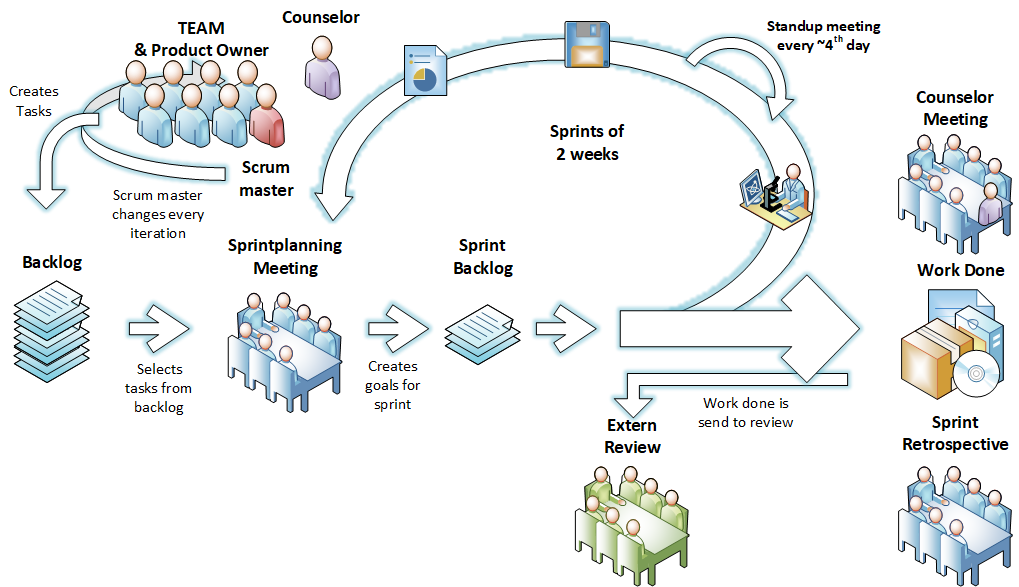
\includegraphics[width=\textwidth]{Processdokument/graphics/Scrum_usage.png}
    \caption{Brugen af Scrum i teamet}
    \label{fig:Scrum_usage}
\end{figure}
Af figur \ref{fig:Scrum_usage} ses det, hvordan gruppen er deres egne Product Owners, hvordan de laver tasks til backloggen og står for sprint planlægningsmødet. Det ses også at Sprints har en varighed af 2 uger, samt at der er Standup meeting ca. hver 4. dag. Her ses også at noget af det arbejde, der bliver færdiggjort bliver sendt til ekstern review af den anden gruppe, og at der afholdes møder med vejleder. Rolen som Scrum Master går også på tur efter hvert sprint.
%Hvad har vi lært af Scrum. Hvad virkede, hvad virkede ikke, hvad var svært, hvad var let?
\\\\Igennem de forrige beskrivelser af hvert enkelt sprint ses det, hvordan der er blevet eksperimenteret med forskellige redskaber i forbindelse med Scrum. Der udtages de vigtigste erfaring i forhold til dette. Det første der gavnede gruppen meget var introduktionen af \textbf{Demoer og Sprint mål} i udviklingen. Til at starte med resulterede planlægningen ikke i noget målbart. Det hjalp derfor udviklingen meget at introducere sprint mål, der kunne fremvises og hvor der kunne siges, at det her blev opnået i sprintet. Derudover virkede \textbf{Risikoanalyse} også som et godt redskab i Scrum udviklingen. Det var op til de enkelte i gruppen at specificere risikoer i forbindelse med projektet, der skulle tages op på vejledermødet. Disse risikoer blev diskuteret og taget hånd om i Sprint planlægningen. Der var også redskaber i forbindelse med Scrum, der virkede godt lige fra start. Det er \textbf{Retrospektiv}, \textbf{Scrumboard}(Selvom anvendelsen af dette forbedredes undervejs), \textbf{StandUp-meeting} og \textbf{Sprintplanlægning}.


\subsection{Udviklingsværktøjer fra 2. Semester}
\subsubsection{Introduktion}
I dette afsnit beskrives de udviklingsværktøjer, der blev genanvendt fra 2. semester. Det drejer sig mere specifikt om ASE-udviklingsmodellen, V-modellen og SysML.
\subsubsection{ASE-modellen}
ASE modellen er en model introduceret på 2. semester, der kan anvendes til at udvikle et system bestående af hardware og software på en struktureret måde. ASE-modellen\footnote{Vejledning til udviklingsprocessen for projekt2} ses i figur \ref{fig:ASE_model}.
\begin{figure}[H]
    \centering
    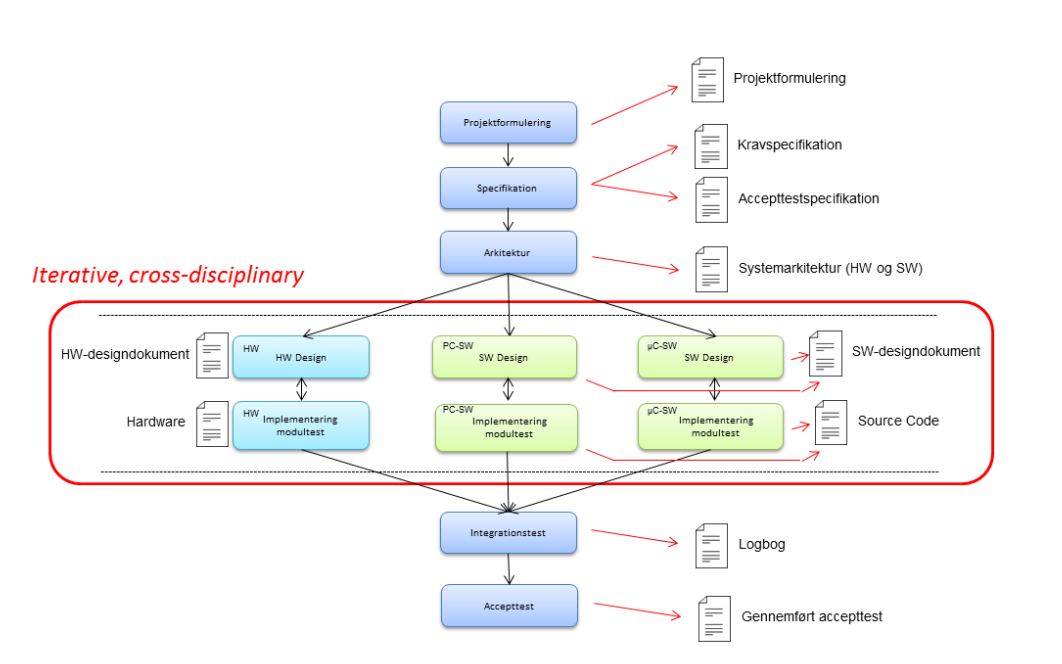
\includegraphics[width=\textwidth]{Processdokument/graphics/ASE_model.png}
    \caption{ASE-udviklingsmodel}
    \label{fig:ASE_model}
\end{figure}
I vores projekt danner ASE-modellen den overordnede struktur for, hvordan systemet er udviklet og beskriver den generelle proces. Processen har fungeret på den måde, at der først blev udarbejdet en formulering om, at projektet omhandlede et interaktivt Beer Pong bord. Herefter blev der lavet en specifikation af de krav, der er for bordet og dens anvendelse, samt opstillet tests for disse.Derefter blev der lavet software og hardware arkitektur, der resulterede i en masse integrationstests af subsystemer. Til sidst laves en accepttest af hele systemet ud fra accepttest-specifikationen. Her er det vigtigt at påpege, den iterative del i midten, der er der, hvor den største anvendelse af Scrum foregår.

\subsubsection{SysML}
Til at udarbejde kravspecifikationen og sytemarkitekturen blev der anvendt SysML, som er et analyse- og design-redskab til, hvilke diagrammer der skulle laves og hvordan. Her anvendtes en modificeret udgave, der passer til de diagrammer, der har optrådt i 2. semester kurset \textit{Indledende System Engineering}. Den modificerede anvendelse af SysML kan ses i figur \ref{fig:Sysml_usage}.
\begin{figure}[H]
    \centering
    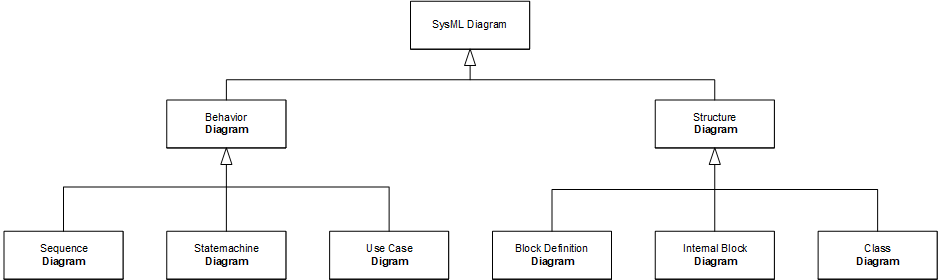
\includegraphics[width=\textwidth]{Processdokument/graphics/Sysml_usage.png}
    \caption{Brugen af SysML i projektet}
    \label{fig:Sysml_usage}
\end{figure}

Af figur \ref{fig:Sysml_usage} ses det, at Sekvens-, Statemachine- og Use Case-diagrammer bruges til at beskrive opførelsen af systemet, hvor Block Definition Diagram og Internal Block Diagram bruges til at beskrive strukturen af systemet. Class diagram fra UML er også inkluderet under struktur, da den beskriver strukturen af software, samt relationen mellem de forskellige klasser. 


\section{Projektledelse}
Scrum Master har stået for ledelsen i det pågældende sprint i forbindelse med styring af gruppen til planlægningen og under sprintet. 
\\Når der skulle tages store beslutninger angående systemet, så blev det gjort på demokratisk vis. De små beslutninger f.eks. beslutnigner angående teknologier og beslutninger i de enkelte delmoduler blev besluttet af dem der arbejdede og havde sat sig ind i modulet.

\section{Arbejdsfordeling}
En af de gode ting ved Scrum er, at man kan påtage sig mange forskellige opgaver inden for mange forskellige områder i et projekt. Dette er umiddelbart ikke realiteten, da mange af de ting, der skal laves på et projekt kræver eksperter inden for flere specifikke områder. Det kan umiddelbart være svært at arbejde på noget hardware eller kode, da man først skal sætte sig ind i teknologien bag det. Muligheden for at sætte sig ind i teknologierne er der, da projektet er så gennemdokumenteret som muligt, men ressourcerne er der måske ikke i det, det kræver en del ressourcer at sætte sig i en ny teknologi. Det skal dog siges at de forskellige i gruppen har været inde over de forskellige dele og teknologier, omend det måske er overfladisk for at reviewe noget kode, udregninger til hardware eller forbindelser mellem modulerne. Derfor er der lavet en overordnet arbejdsfordeling som kan ses i tabel \ref{table_work_distribution}.
\begin{table}[H]
\centering
\begin{tabular}{|L{0.2\textwidth}|L{0.7\textwidth}|}
\hline
\textbf{Navn} & \textbf{Overordnet Arbejdsområde} \\ \hline
Nikolaj & Hardware og hardwarenær software \\ \hline
Tristan &  RPi softwaresystem (Controller, Kommunikation og Integration)\\ \hline
Mathias & Controller software boundary  \\ \hline
Edward &  \\ \hline
Martin G.J & Software boundaries \\ \hline
Martin F. & Software  \\ \hline
Aaron & Status LED'er, Ballcount sensor og dispensering af bolde \\ \hline
Marcus & Interaktivt lys under kopper og proces \\ \hline
\end{tabular}
\caption{Overordnet arbejdsfordeling i gruppen}
\label{table_work_distribution}
\end{table}
Her er det vigtigt at pointere dette kun er det overordnede billede af arbejdsfordelingen, da der også har lagt arbejde i mange andre forbindelser af projektet.

\section{Planlægning}
\subsection{Planlægning af projektet}
I starten af projektet blev der lavet en overordnet tidsplan, der løbende blev opdateret i forhold til dokumenter, der blev færdiggjort og milestones, der blev opnået. Denne tidsplan ses i figur \ref{fig:projekt_schedule}.
\begin{figure}[H]
    \centering
    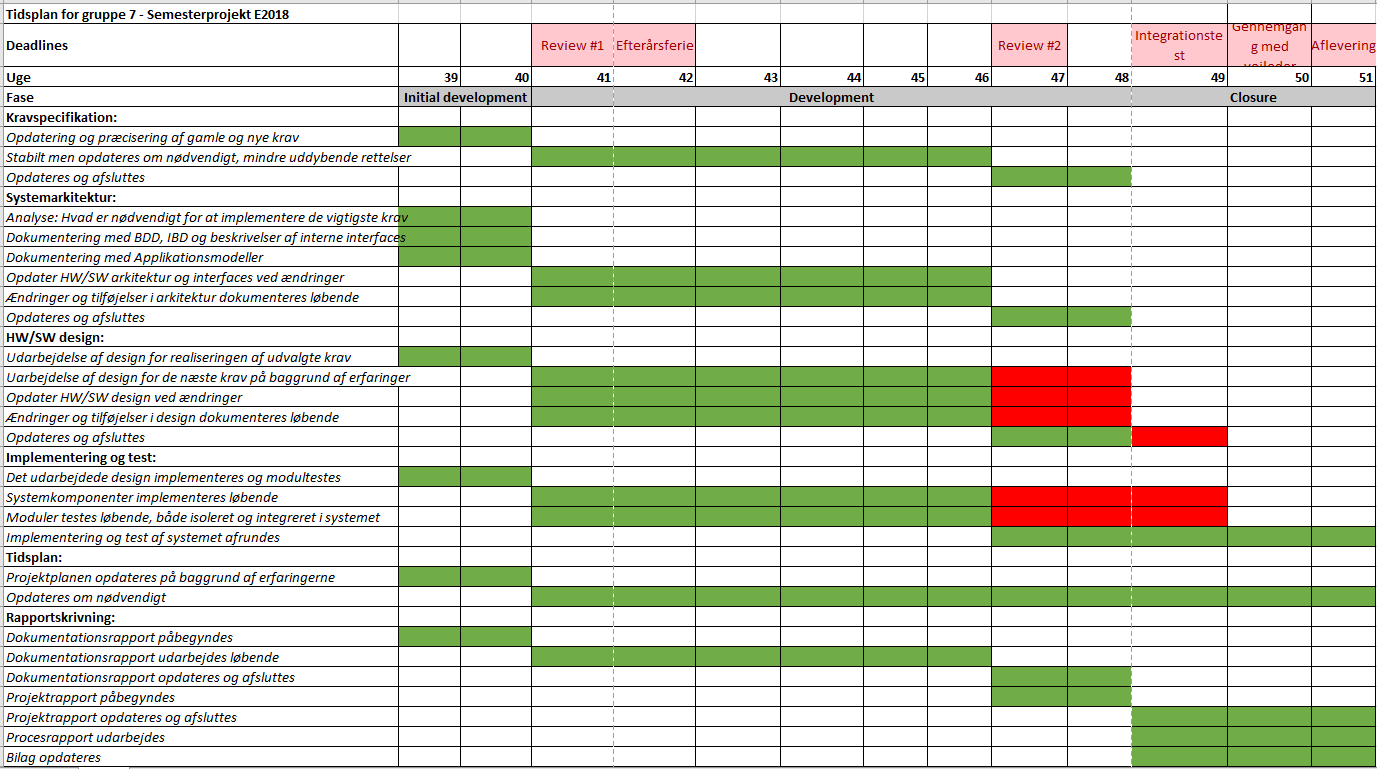
\includegraphics[width=\textwidth]{Processdokument/graphics/Tidsplan.png}
    \caption{Tidsplanen for projektet}
    \label{fig:projekt_schedule}
\end{figure}
En ting der er vigtig at lægge mærke til ved figur \ref{fig:projekt_schedule} er, hvordan mange af delene strækker sig over forholdsvis mange uger. Det er af den grund at der blev arbejdet iterativt, hvilket for eksempel gjorde, at der blev vendt tilbage til mange af dokumenterne for eventuelle rettelser og tilføjelser. 

\subsection{Iterativ Planlægning}
Da der som sagt er blevet arbejdet iterativt, så skulle der også planlægges ting iterativt. Det kan for eksempel være, hvad fokus er for dette sprint, hvilke mål skal der være og så videre. I starten af projektet var mange af disse mål meget forudbestemte ud fra deadlines som review. Det hænger sammen med den dokumentation, der skulle færdiggøres til deadlinen. Da udviklingsfasen så påbegyndtes blev planlægningen af sprintet en mere fælles rolle, som det også var meningen.


\section{Møder} 
\subsection{Introduktion}
I dette afsnit beskrives overordnet set de møder, der har været i forbindelse med projektet. Møderne vil ikke beskrives hver især, men der henvises til Vejledermøde- og Gruppemøde-dokumentet. Til internt at holde styr på møder blev, der anvendt Google Calendar. Den blev anvendt over Redmine kalenderen, da den kunne synkroniseres med hver enkelts personlige kalender, og den var nemmere at tilføje og rette ting i. I de følgende afsnit vil de forskellige typer af møder beskrives overordnet.
\subsection{Vejledermøder}
Den første type af møder, der beskrives er vejledermødet. Til denne type møde var det Scrum Masters ansvar at samle et dokument med fokuspunkter for mødet og få det sendt til vejleder, senest en dag før mødet. Mødet havde en generel struktur af at først blev der stillet forskellige spørgsmål i forbindelse med projektet, hvor efter der blev lavet en risikoanalyse af hvad gruppen generelt synes var en risiko for ikke at nå i mål. Til mødet var en referent, der gik på tur, som stod for at nedskrive et referat i bunden af møde indkaldelsen, så det hele var samlet et sted. Dette møde fungerede i Scrum terminologi som Scrum Review-mødet.
\subsection{Gruppemøder}
Dette var de interne møder i gruppen, hvor der blev arbejdet på projektet. I starten af projektet blev gruppemøderne brugt meget til at gennemgå forskellige dokumenter eller diagrammer i fællesskab, for at skabe en fælles forståelse for systemet og samtidig sikrer at kvaliteten på dokumenterne var høj fra en start af. Senere hen i processen udviklede disse gruppemøder sig mere til at arbejde på implementeringsaspekter i fællesskab, samt at sikrerer at de indbyrdes interfaces spillede sammen. Derudover blev de også brugt til at spørge om hjælp, og komme med review på det arbejde andre havde lavet.
\subsection{Review}
Reviewet var de to planlagte møder, hvor der skulle laves et review af en anden gruppes materiale og de samtidig lavede review af det materiale de var givet. Gruppen der blev tildelt var gruppe 10, der lavede et projekt omkring en robot arm. Til at lave review af den anden gruppe blev udvalgt 3 gruppemedlemmer, som havde til ansvar at lave review af det udleverede materialle og sammensætte et dokument af deres review.  Mødets forløb var at først lavede den ene gruppe et review, mens den anden gruppe sugede den konstruktive kritik til sig uden at stille for mange spørgsmål og derefter byttedes rollerne. 

\section{Konflikthåndtering}

\section{Referenceliste}


\end{document}
